\documentclass[aspectratio=43]{beamer}
% \documentclass[aspectratio=169]{beamer}

% Title --------------------------------------------
\title{Treatment Effect Estimation with Geocoded Microdata}
\subtitle{}
\date{\today}
\author{Kyle Butts}

% Margins ----------------------------------------------------------------------

\usepackage[margin=1.25in]{geometry}

% AMS --------------------------------------------------------------------------

\usepackage{amsmath}
\usepackage{amsfonts}
\usepackage{amsthm}
\usepackage{graphicx}


% Line Spacing -----------------------------------------------------------------

\renewcommand{\baselinestretch}{1.5}


% Font -------------------------------------------------------------------------

\usepackage[T1]{fontenc}
\usepackage[default]{lato}
% \usepackage[utopia, varg]{newtxmath}
% \renewcommand{\rmdefault}{futs} % Utopia as text font 

% Small adjustments to text kerning
\usepackage{microtype}

% Remove annoying over-full box warnings
\vfuzz2pt 
\hfuzz2pt


% Tikz support -----------------------------------------------------------------

\usepackage{tikz}


% Color Palette ----------------------------------------------------------------

\usepackage{xcolor}

% https://www.materialpalette.com/colors
\definecolor{dark-maroon}{HTML}{5D0F0D}
\definecolor{navyblue}{HTML}{0A3044}

% https://www.viget.com/articles/color-contrast/
\definecolor{purple}{HTML}{5601A4}
\definecolor{navy}{HTML}{0D3D56}
\definecolor{ruby}{HTML}{9a2515}
\definecolor{alice}{HTML}{107895}
\definecolor{daisy}{HTML}{EBC944}
\definecolor{coral}{HTML}{F26D21}
\definecolor{kelly}{HTML}{829356}
\definecolor{cranberry}{HTML}{E64173}
\definecolor{jet}{HTML}{131516}
\definecolor{asher}{HTML}{555F61}
\definecolor{slate}{HTML}{314F4F}


% Hyperlinks -------------------------------------------------------------------

\usepackage{hyperref}
\hypersetup{
    colorlinks= true,
    citecolor= dark-maroon,
    linkcolor= dark-maroon,
    filecolor= dark-maroon,      
    urlcolor= dark-maroon,
}


% Citations --------------------------------------------------------------------

% note, natbib provides better hyperlinking
\usepackage{natbib}
\bibliographystyle{econ-aea}
% How to display multiple in \citet{}
\setcitestyle{comma,aysep={}}

% Define Theorems --------------------------------------------------------------

% Put proper spacing after Theorem #. 
\newtheoremstyle{spacing}
{}%          Space above, empty = `usual value'
{}%          Space below
% {\itshape}%  Body font
{}%  Body font
{}%          Indent amount (empty = no indent, \parindent = para indent)
{\bfseries\color{navyblue}}% Thm head font
{.\ }%         Punctuation after thm head
{2.5mm}%  Space after thm head: \newline = linebreak
{}%          Thm head spec

% note, theorem is the name that goes in \begin{} and Theorem is the name displayed as Theorem 1
\theoremstyle{spacing}
\newtheorem{theorem}{Theorem}
\newtheorem{proposition}{Proposition}
\newtheorem{assumption}{Assumption}
\newtheorem{remark}{Remark}
\newtheorem{example}{Example}


% Custom Math Definitions ------------------------------------------------------

\global\long\def\expec#1{\mathbb{E}\left[#1\right]}%
\newcommand{\condexpec}[2]{\mathbb{E}\left[#1 \ \vert \ #2\right]}
\global\long\def\prob#1{\mathbb{P}\left[#1\right]}%
\global\long\def\var#1{\mathrm{Var}\left[#1\right]}%
\global\long\def\cov#1{\mathrm{Cov}\left[#1\right]}%
\global\long\def\one{\mathbf{1}}%


% Titlepage --------------------------------------------------------------------

% \maketitle
\usepackage{titling}
\usepackage{setspace}

% title
\pretitle{\begin{spacing}{1}\begin{flushleft}\huge}
\posttitle{\end{flushleft}\end{spacing}\vspace{-5mm}}
% author, note don't use \and 
\preauthor{\begin{flushleft}\LARGE}
\postauthor{\end{flushleft}\vspace{-7.5mm}}
% date
\predate{\begin{flushleft}\Large\color{asher}}
\postdate{\end{flushleft}\vspace{-5mm}}

% Abstract
\renewenvironment{abstract}
 {\noindent\rule{\linewidth}{.5pt}\noindent}
 {\noindent\rule{\linewidth}{.5pt}}

% alternative abstract
% \renewenvironment{abstract}
% {
%   \centerline {\large \bfseries \scshape \color{navyblue} Abstract}
%   \begin{quote}
% }
% {\end{quote}}


% Section and Subsection Styling -----------------------------------------------

\usepackage[explicit]{titlesec}

\titleformat{\section}
  {\large \bf \color{navyblue}}
  {\thesection \,---}
  {0.25em}
  {#1}
  
\titleformat{\subsection}
  {\fontsize{11}{10}\it}
  {\thesubsection.}
  {1em}
  {#1}


% Footnote ---------------------------------------------------------------------

% Spacing between footnotes on same page
\addtolength{\footnotesep}{1mm}

% Space after footnote number
\let\oldfootnote\footnote
\renewcommand\footnote[1]{\oldfootnote{\ #1}}

% No footnote line
\renewcommand\footnoterule{}

% No supsercript in footer
\makeatletter
\renewcommand\@makefntext[1]{%
    \parindent 1em \noindent
    \hb@xt@1.8em{\hss\normalfont\@thefnmark.\hfill}#1
  }
\makeatother




% Enumerate/Itemize ------------------------------------------------------------

\usepackage{enumitem}
\setitemize{labelindent=0.5em,labelsep=0.25cm,leftmargin=*}
\setenumerate{labelindent=0.5em,labelsep=0.25cm,leftmargin=*}


% Table and Figure labelling ---------------------------------------------------

\usepackage{caption}

\DeclareCaptionLabelSeparator{threedash}{\,---\,}
\DeclareCaptionFont{navyblue}{\color{navyblue}}
\DeclareCaptionFont{jet}{\color{jet}}
\captionsetup[table]{format=plain, labelsep=threedash, font={navyblue, bf}}
\captionsetup[figure]{format=plain, labelsep=threedash, font={navyblue, bf}}

% Alternative: Left align captions
% \captionsetup[table]{labelfont=it, textfont={navyblue, bf}, labelsep=newline, justification=raggedright, singlelinecheck=off}
% \captionsetup[figure]{labelfont=it, textfont={navyblue, bf}, labelsep=newline, justification=raggedright, singlelinecheck=off}

% multifigure with \caption
% \begin{subfigure}\caption{} \end{subfigure}
\usepackage{subcaption}
\captionsetup[subfigure]{format=plain, font={jet, footnotesize, bf}}


% Tables -----------------------------------------------------------------------

% Fix \input with tables
% \input fails when \\ is at end of external .tex file
\makeatletter
\let\input\@@input
\makeatother

% Make tables/figures wider than \textwidth using:
% \begin{adjustbox}{width = 1.2\textwidth, center}
% \end{adjustbox}
\usepackage{adjustbox}

% Slighty more spacing between rows
\usepackage{array}
\renewcommand\arraystretch{1.25}

% Table with easy to use footnotes
% \begin{threeparttable}
%    \begin{tabular} ... \end{tabular}
%    \begin{tablenotes}
%        \item \textit{Notes.}
%    \end{tablenotes}  
% \end{threeparttable}
\usepackage[flushleft]{threeparttable}
\setlength\labelsep{0pt}

% \toprule, \cmidrule, \bottomrule
\usepackage{booktabs}

% If tables are too narrow, fill columns using:
% \begin{tabularx}{\linewidth}{cols}
% col-types: X - center, L - left, R -right
% If you want relative scale for columns: 
% >{\hsize=.8\hsize}X/L/R
\usepackage{tabularx}
\newcolumntype{L}{>{\raggedright\arraybackslash}X}
\newcolumntype{R}{>{\raggedleft\arraybackslash}X}
\newcolumntype{C}{>{\centering\arraybackslash}X}

% Landscape table 
% \begin{landscape} \pagestyle{lscaped} table... \end{landscsape}
% \usepackage{pdflscape} - rotates page left-side up in pdf
% \usepackage{lscape} - does not rotate page, only figure/table

\usepackage{pdflscape}

% For landscape, fix page number location
\usepackage{fancyhdr}
\fancypagestyle{lscaped}{%
    \fancyhf{}
    \renewcommand{\headrulewidth}{0pt}
    \textnormal
    \fancyfoot{%
        \tikz[remember picture,overlay]
        \node[outer sep=2.5cm,above,rotate=90] at (current page.east) {\thepage};
    }
}
  

% ------------------------------------------------------------------------------


\newcommand{\dist}{\text{Dist}}

% Set-up Bibliography ------------------------------
\addbibresource{references.bib}

\begin{document}

% ------------------------------------------------------------------------------
\maketitle
% ------------------------------------------------------------------------------

\begin{frame}{Motivation}

    Treatment often isn't assigned to groups of individuals (e.g. counties), but rather to specific locations

    \begin{itemize} 
        \item Environmental: Local pollutants \citepcolor{Marcus_2021,Currie_Davis_Greenstone_Walker_2015}, shale gas discovery \citepcolor{Muehlenbachs_Spiller_Timmins_2015}
    
        \item Urban: foreclosures \citepcolor{Gerardi_Rosenblatt_Willen_Yao_2015,Campbell_Giglio_Pathak_2011}, abandon lot cleanups \citepcolor{South_Hohl_Kondo_2018}, apartment construction \citepcolor{Asquith_Mast_Reed_2021} 
    \end{itemize}
\end{frame}

\setbeamercovered{transparent}

\begin{frame}{Identification of Treatment Effects}
    Difference-in-differences is often used to estimate treatment effects. How do you choose a control group?
    \vspace{2.5mm}
    
    \begin{enumerate}
        \item<1> Find alternative treatment locations to serve as a control group. For example propensity score match census blocks and use observations in blocks likely to receive treatment but did not.
            
            \begin{itemize}
                \item Problem if areas actually treated are targeted due to contemporaneous shocks to trends.
            \end{itemize}
        
        \item<2> Compare observations very near to treatment, ``the treated'', to observations just slightly further away, ``the control''.
            
            \begin{itemize}
                \item Identification allows treatment to be targeted due to `neighborhood` trends but not targeted for differential trends `within` the neighborhood.
            \end{itemize} 
    \end{enumerate}
\end{frame}


% Example Quotes
\begin{frame}{Examples of Identification Discussion}
    \citetcolor{Linden_Rockoff_2008} look at the arrival of sexual offenders on neighborhood prices.They compare home sales \textbf{within 0.1 mile (about 2 city blocks) to home sales between 0.1 - 0.3 miles}. 

    \vspace{2.5mm}
    \begin{quote}
        ``This framework would be compromised only if sex offenders
        consistently moved into properties near which a localized disamenity was likely to emerge.''
    \end{quote}
\end{frame}


\begin{frame}{Examples of Identification Discussion}
    \citetcolor{Marcus_2021} considers leaking underground petroleum storage tanks that affect hyper-local drinking water. Look at long-run outcomes of children exposed to petroleum pollution

    \vspace{2.5mm}
    \begin{quote}
        ``I find that low-SES mothers are more likely to live near pollution sites. ... The remaining threat to identification is time-varying unobservable characteristics (e.g. local economic conditions) that vary systematically with the observed leak timing. To address
        this concern, I compare mothers \textbf{within two small radii of the leaking site, 300 and 600 meters.}''
    \end{quote}
\end{frame}


\begin{frame}{Problem} 
    The central problem is how do you chose the radii of the two rings?

    \begin{itemize}
        \item Does treatment effects stop at 0.1 miles? 0.2 miles? 0.3 miles?
        \item How far constitutes the "neighborhood" that control units can be in?
    \end{itemize}
\end{frame}

\begin{frame}{Contribution}
    \begin{enumerate}
        \item I formalize the identification strategy in an econometric framework.
        
        \item Define what assumptions are needed to identify estimands: `parallel trends' within control ring and correct treatment effect cutoff distance.
        
        \item I propose a new estimator that relaxes the correct treatment effect cutoff assumption using new work on non-parametric series estimators \citetcolor{Cattaneo_Crump_Farrell_Feng_2019,Cattaneo_Farrell_Feng_2019}.
    \end{enumerate}
\end{frame}


% ----------------------------------------------------------------------------
\section{Example of Problems}
% ----------------------------------------------------------------------------

\imageframe{../../figures/slides-example_dgp.pdf}
\imageframe{../../figures/slides-example_a.pdf}
\imageframe{../../figures/slides-example_b.pdf}
\imageframe{../../figures/slides-example_c.pdf}
\imageframe{../../figures/slides-example_d.pdf}

% ----------------------------------------------------------------------------
\section{Theory}
% ----------------------------------------------------------------------------

\begin{frame}{Model for Outcomes}{Setup}
    Units $i$ have locations $(x_i, y_i)$. Treatment turns on between the two periods $t = 0, 1$ at point $(\bar{x}, \bar{y})$. Therefore units vary in $\dist_i$, their distance to treatment. We have an iid panel sample. 


    \vspace{2.5mm}
    Outcomes are given by:

    $$
    Y_{it} = \underbrace{\color{coral} \tau(\dist_i) \one_{t = 1}}_{\text{Treatment Effect Curve}} + \mu_i + \underbrace{\color{kelly}\lambda(\dist_i) \one_{t=1}}_{\text{Counterfactual Trend}} + \varepsilon_{it},
    $$

    \vspace{2.5mm}
    where we assume $\varepsilon_{it} \perp \dist_i$.
\end{frame}

\begin{frame}{Model}{Estimand}
    Estimand of interest: 
    $$
    \bar{\tau} = \condexpec{ \tau(\dist_i) }{ \tau(\dist_i) > 0 }
    $$

    This is just the average treatment effect on those affected by treatment.
\end{frame}

\begin{frame}{Model}{First-Differences}
    Taking first differences, we have:

    $$
    \Delta Y_{it} = { \color{coral} \tau(\dist_i)} + {\color{kelly} \lambda(\dist_i)} + \Delta \varepsilon_{it}
    $$

    With no additional assumptions, the {\color{coral} treatment effect curve} and the {\color{kelly} counterfactual trend} are not seperately identifiable.
\end{frame}

\begin{frame}{Model}{Assumptions}
    \textbf{\color{alice} Assumption:} {\color{asher} Local Parallel Trends}

    For a distance $d_c$, local parallel trends hold if ${\color{kelly} \lambda}$ is constant for $0 < d < d_c$.

    \vspace{5mm}
    \textbf{\color{alice} Assumption:} {\color{asher} Average Parallel Trends}

    For a distance $d_c$ and $d_t$, average parallel trends hold if

    $$\condexpec{{\color{kelly} \lambda_d}}{0 \leq d \leq d_t} = \condexpec{{\color{kelly} \lambda_d}}{d_t < d \leq d_c}$$

    \pause
    \begin{itemize}
        \item {\color{asher} Average Parallel Trends} is a milder assumption, but usually researchers justify the method by {\color{asher} Local Parallel Trends}.
    \end{itemize}
\end{frame}

\begin{frame}{Model}{Assumptions}
    \textbf{\color{alice} Assumption:} {\color{asher} Correct Treatment Effect Cutoff}

    A distance $d_t$ satisfies this assumption if for all $d \leq d_t$, ${\color{coral} \tau(d)} > 0$ and for all $d > d_t$, ${\color{coral} \tau(d)} = 0$.

    \pause
    \begin{itemize}
        \item This is difficult to know!!!
        
        \item Later on, I show how to relax this assumption under {\color{asher} Local Parallel Trends}
    \end{itemize}
\end{frame}


\begin{frame}{Estimator}
    For a given $d_t$ and $d_c$, we define the treated and control groups as:
    
    $$\mathcal{D}_t = \{ i \ : \ \dist_i \leq d_t \}; \quad \mathcal{D}_c = \{ i \ : \ d_t < \dist_i \leq d_c \}$$
    
    
    On the sample $\mathcal{D}_t \cup \mathcal{D}_c$, the following regression is run:
    
    $$
        \Delta Y_{it} = \beta_0 + \beta_1 \one_{i \in D_t} + u_{it}
    $$

    $\hat{\beta}_1$ is the difference-in-differences estimate
    
\end{frame}

\begin{frame}{Identification}{Decomposition of Ring Method}

    \begin{enumerate}
        \only<1>{
        \item[(i)]The estimate of $\beta_1$ has the following expectation:
        {\footnotesize
            \[ 
                \expec{\hat{\beta}_1} = 
                \underbrace{\condexpec{\tau(\dist)}{\mathcal{D}_t} - \condexpec{\tau(\dist)}{\mathcal{D}_c} }_{\text{Difference in Treatment Effects}} 
                + \underbrace{\condexpec{\lambda(\dist)}{\mathcal{D}_t} - \condexpec{\lambda(\dist)}{\mathcal{D}_c} }_{\text{Difference in Trends}}.
            \]
        }
        }
        
        \only<2>{
        \item[(ii)] More, if $d_c$ satisfies {\color{asher} Local Parallel Trends} (or {\color{asher} Average Parallel Trends}), then
        {\footnotesize
            \[ 
                \expec{\hat{\beta}_1} = 
                \underbrace{\condexpec{\tau(\dist)}{\mathcal{D}_t} - \condexpec{\tau(\dist)}{\mathcal{D}_c} }_{\text{Difference in Treatment Effects}}.
            \] 
        }
        }
        
        \only<3>{
        \item[(iii)]<3> If $d_c$ satisfies {\color{asher} Local Parallel Trends}(or {\color{asher} Average Parallel Trends}) and $d_t$ is the correct distance cutoff, then
        {\footnotesize
            \[ 
                \expec{\hat{\beta}_1} = \bar{\tau}.
            \]
        }
        }
    \end{enumerate}
    
\end{frame}


% ----------------------------------------------------------------------------
\section{Improved Estimator}
% ----------------------------------------------------------------------------

\begin{frame}{Improved Estimator}{Difficulties with Assumptions}

In most cases, it is hard for a researcher to know ad-hoc what the correct $d_t$ is to satisfy the correct cutoff assumption.

\vspace{5mm}
There is a \emph{data-driven} way to estimate treatment effect curve, $\tau(\dist)$ without specifying $d_t$.
\begin{itemize}
    \item The method uses a non-parametric partition-based estimator proposed by \citetcolor{Cattaneo_Farrell_Feng_2019}.
\end{itemize} 
    
\end{frame}


\imageframe{../../figures/slides-example_did.pdf}
\imageframe{../../figures/slides-example_partition.pdf}

\begin{frame}{Improved Estimator}{Advantages}

    \begin{enumerate}
        \item Estimates a treatment effect curve rather than an average effect
        
        \begin{itemize}
            \item E.g. bus stop is built. Negative effects very close, positive effects slightly further away. Average effect $\approx 0$.
        \end{itemize}

        \pause
        \item Gives an informal visual test of {\color{asher} Local Parallel Trends}
  
        \begin{itemize}
            \item Curve should level off around zero
        \end{itemize}
    \end{enumerate}
\end{frame}

% ----------------------------------------------------------------------------
\section{Application}
% ----------------------------------------------------------------------------

\begin{frame}{Application}{\citet{Linden_Rockoff_2008}}
    \citetcolor{Linden_Rockoff_2008} look at the local effects on home prices of a registered sex offender moving into the neighborhood. 
    
    \begin{itemize}
        \item They compare homes within 0.1 miles of the offender's home to control units between 0.1 mile and 0.3 miles. 
        
        \emph{Is 0.1 mile the correct cutoff?}
        
        \item They assume that treatment effect is constant for being on the same block and being a few blocks away. 
        
        \emph{Is this a assumption correct?}
    \end{itemize}
\end{frame}

\begin{frame}
    \begin{figure}
        \caption{Effects of Offender Arrival on Home Prices \citep{Linden_Rockoff_2008}}
        \centering
        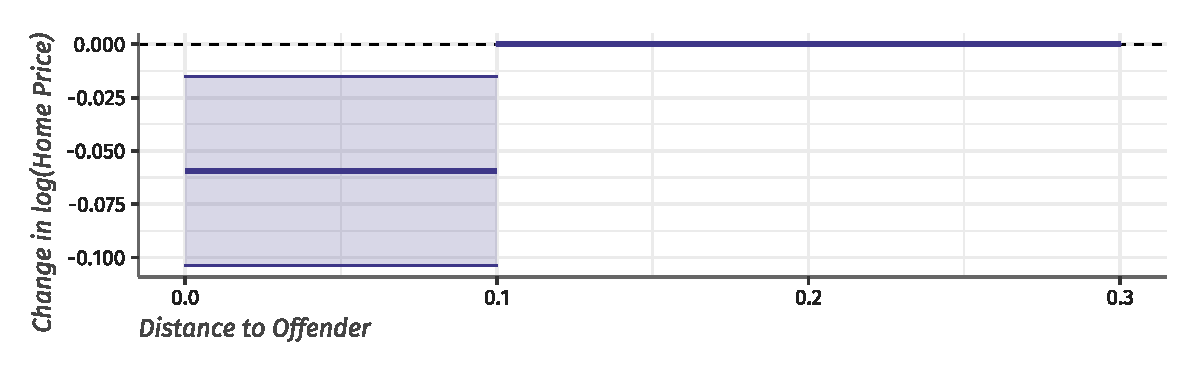
\includegraphics[width=\textwidth]{../../figures/linden_rockoff_did.pdf}
    \end{figure}
    \vspace{-5mm}
    \begin{figure}
        \vspace{-5mm}
        \centering
        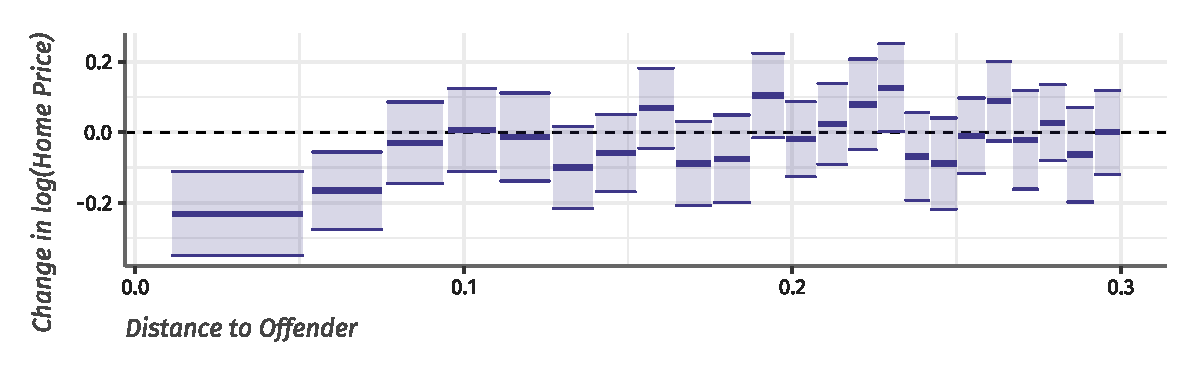
\includegraphics[width=\textwidth]{../../figures/linden_rockoff.pdf}
    \end{figure}
\end{frame}



\begin{frame}{Conclusion}

The standard ``indicator'' version of the rings method requires knowledge of the treatment effect cutoff.

\vspace{5mm}
I proposed an estimator that:
    \begin{enumerate}
        \item Relaxes this assumption
        \item Allows estimation of the treatment effect curve instead of average effect
    \end{enumerate}

\vspace{5mm}
\begin{center}
\color{alice}{Thank you!}
\end{center}
    
\end{frame}



% ----------------------------------------------------------------------------
\begin{frame}[allowframebreaks]{References}
    \printbibliography
\end{frame}
% ------------------------------------------------------------------------------

\end{document}